\begin{questions}
\question{
Why don't vector $\vec{a}$ and $\vec{b}$ form a Bravais lattice?
}
\begin{solution}
  In this case such vectors don't form a Bravais Lattice because a Bravais lattice must look the same for every $\vec{R} = n_1\vec{a} + n_2 \vec{b}$, with $n_1,n_2\in \mathbb{Z}$, and this is not the case for this choice of primitive vectors.
  For example for the two points depicted in fig. \ref{fig:wrong} the lattice will not look the same
\begin{center}
  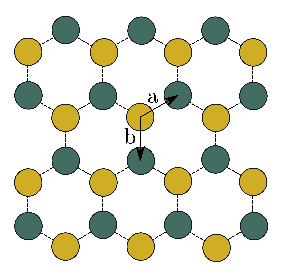
\includegraphics[width=55mm]{original}
\end{center}
\captionof{figure}{Example of two points for which the lattice is not going to look the same}\label{fig:wrong}

\end{solution}

\question{
How can one construct a Bravais lattice for this system?
}
\begin{solution}

We can actually create a Bravais lattice if we change the primitive vectors and define the basis as shown in fig. \ref{new}
\clearpage
\begin{center}
  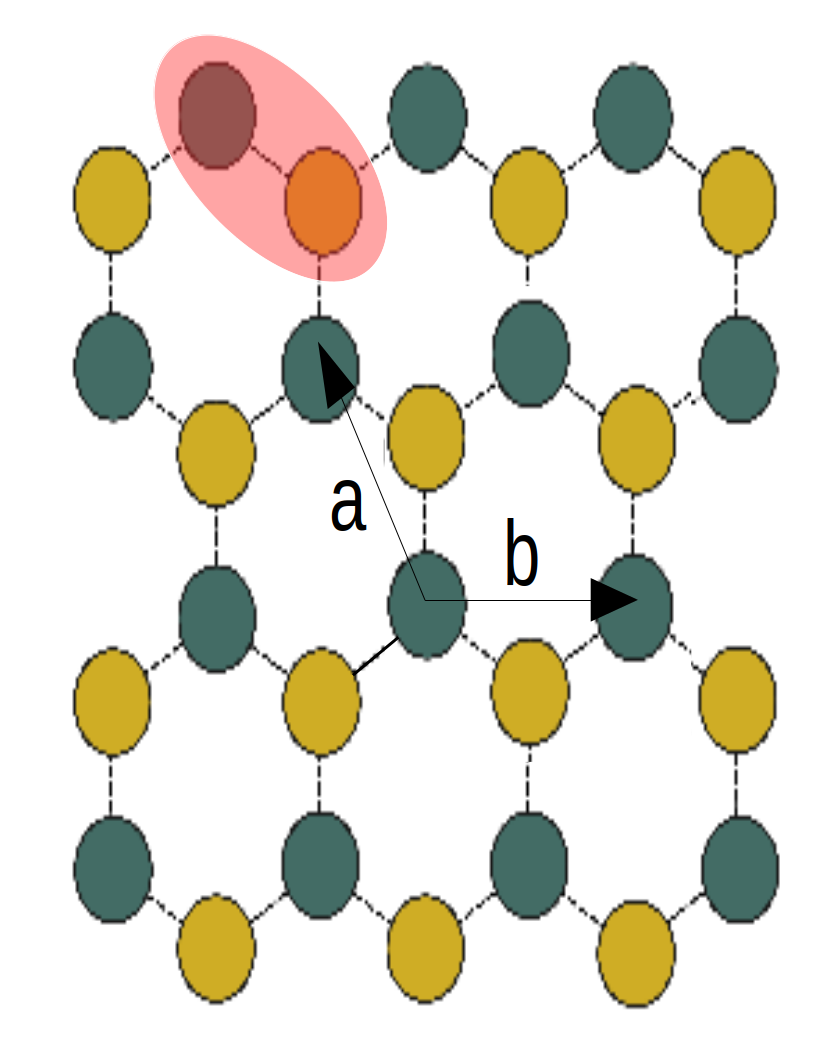
\includegraphics[width=45mm]{lat}
\end{center}

\captionof{figure}{New primitive vectors and new basis to turn the honeycomb into a Bravais lattice. The new vectors are also named $\vec{a}, \vec{b}$ and the basis is enclosed on the ellipse on the top left part of the image.}\label{new}

\end{solution}


\question{Construct the Wigner-Seitz cell for this Bravais lattice.}
\begin{solution}

  In fig. \ref{voronoi} we can see the construction of the Wigner-Seitz cell. Basically we draw lines between first neighbors. After that we draw the median to the lines drawn on the last step. And finally the cell we are looking for will be the volume comprised inside the medians drawn on the second step.

  \begin{center}
    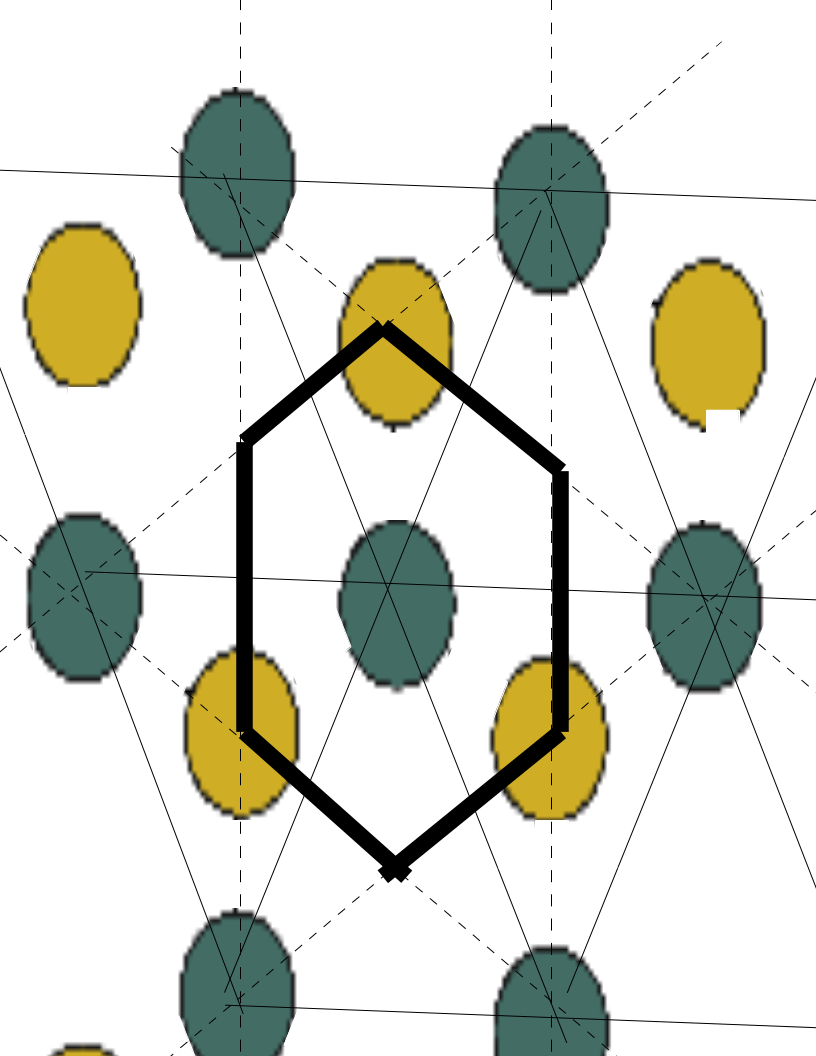
\includegraphics[width=55mm]{voronoi}
  \end{center}

  \captionof{figure}{Wigner-Seitz cell for the our Bravais lattice. The solid thin lines are connections between first neighbors. The dashed lines are the medians to the lines joining first neighbors. The solid wide lines are then the limits of the Wigner-Seitz cell.}\label{voronoi}
\end{solution}

\end{questions}

%
% \begin{center}
%   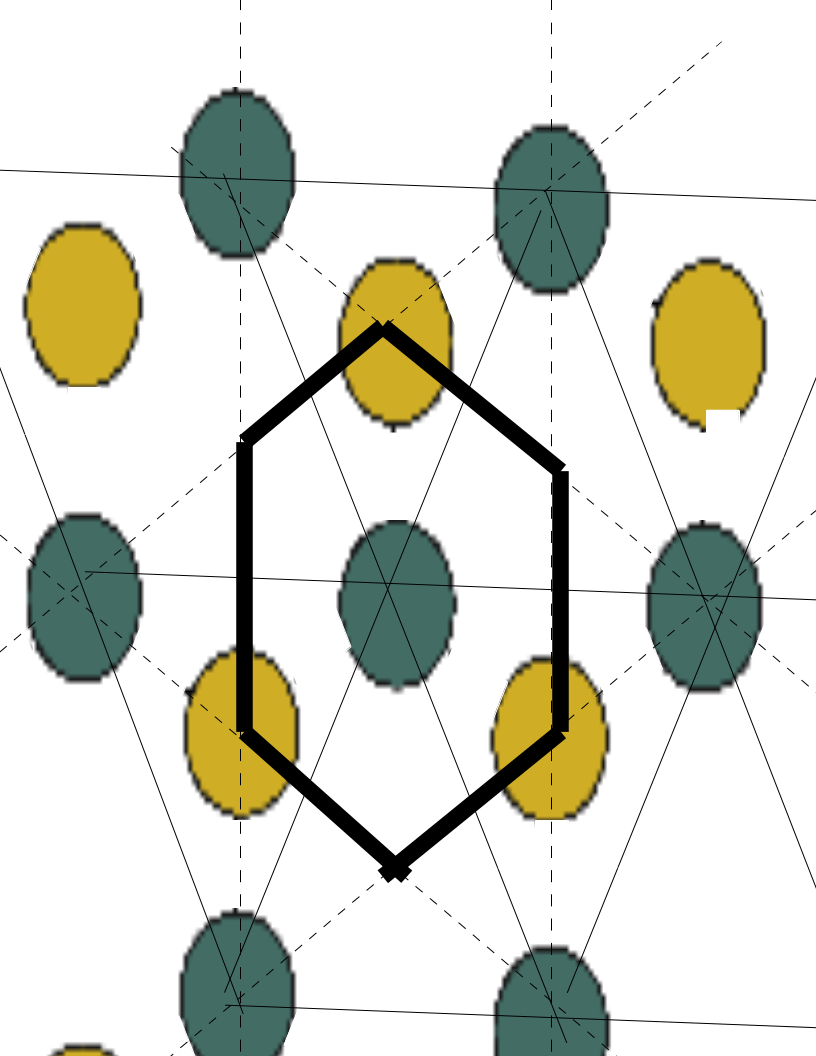
\includegraphics[width=55mm]{voronoi}
% \end{center}
%
% \captionof{figure}{}\label{new}
